\documentclass[DM,authoryear,toc]{lsstdoc}
% lsstdoc documentation: https://lsst-texmf.lsst.io/lsstdoc.html
\input{meta}

% Package imports go here.

% Local commands go here.

%If you want glossaries
%\input{aglossary.tex}
%\makeglossaries

\title{Periodicity Analysis in Alert Production}

% Optional subtitle
% \setDocSubtitle{A subtitle}

\author{%
Anastasios Tzanidakis, Eric Bellm
}

\setDocRef{DMTN-221}
\setDocUpstreamLocation{\url{https://github.com/lsst-dm/dmtn-221}}

\date{\vcsDate}

% Optional: name of the document's curator
% \setDocCurator{The Curator of this Document}

\setDocAbstract{%
The baselined timeseries features to be computed in Alert Production include a Lomb-Scargle periodogram.  We assess the computational and scientific performance of several configurations on simulated alert data.
}


% Change history defined here.
% Order: oldest first.
% Fields: VERSION, DATE, DESCRIPTION, OWNER NAME.
% See LPM-51 for version number policy.
\setDocChangeRecord{%
  \addtohist{1}{YYYY-MM-DD}{Unreleased.}{Anastasios Tzanidakis, Eric Bellm}
}


\begin{document}

% Create the title page.
\maketitle
% Frequently for a technote we do not want a title page  uncomment this to remove the title page and changelog.
% use \mkshorttitle to remove the extra pages

% ADD CONTENT HERE
% You can also use the \input command to include several content files.

\section{Note}
\textcolor{red}{Please note that this DM-technote is currently work in progress, and publicly available. The final findings will be pushed to the DMTN-221 repository in late November of 2022 by Anastasios Tzanidakis.}


\section{Motivation}
The characterization of periodicity from time-series is a fundamental constraint to numerous astrophysical applications. Phenomenologically, estimating the periodicity and its significance can shed light on stellar pulsation theory \citep{Antonello:Antonello81}, distance estimation and mapping of the Galaxy through the period-luminosity relationship \citep{Skowron:Skowron2019}, constraint fundamental parameters of stellar binaries \citep{Farinella:Farinella1979} and stellar rotation \citep{Walkowicz:Walkowicz13}. In the recent decade, the use of periodicity has also been extensively used as a feature to classify variable phenomena \citep{Richards:R13} across the HR diagram. 


Previous work from \cite{2012AJ....144....9O} demonstrate the concept of injection-recovery test for synthetically generated RR Lyrae templates from SDSS using the op$\_$sim version 1.29 cadence strategy. However, no study to date has demonstrated the recovery period distribution of more complex periodic phenomena (i.e eclipsing binaries, quasi-periodic AGN). Here we perform an end-to-end, injection and recovery analysis for multi-band time series to asses the statistical significance of period finding in the context of AP. 


\section{Synthetic Light Curves}
In this study we use the training set Extended LSST Astronomical Time-series Classification Challenge (ELAsTiCC) light curves with a 12 month history that will best mimic the calculations performed for AP. In short, ELAsTiCC is an end-to-end real-time pipeline for generating mock photometric alerts at the expected Legacy Survey of Time and Space (LSST) rate. The photometric alerts will be distributed in real-time to brokers to benchmark classification algorithms. The ELAsTiCC uses the v.1.7 cadence strategy from op$\_$sims. A single detection is based on the DIA performance from DC2. Each light curve include photometric noise using Poisson noise that includes the equivalent area, background noise per unit area, sky and CCD read noise. Most importantly, the ELAsTiCC light curves simulate force photometry alerts which we recommend all time series features to be calculated upon. 
	
	Here we present two classes of periodic sources: RR Lyrae (RRL) and eclipsing binaries (EB). Both RRL's and EB's represent both the extrema of simple and complex periodic sources that will throughly test the underlying ability of the periodogram to find the correct period. Currently, the eclipsing binary sample from ELAsTiCC that was generated from open-source Python package Eclipsing binary Learning and Interactive System (ELISa). the only contains a few hundred simulated binaries. To maximize the use different eclipsing binary stars sampled at different phases, each light curve over a three year photometric history is sampled at some random time and ensures that the maximum baseline is less than 12 months. In Figure \ref{fig:light_curve_demo} we show the typical multi-band AP light curve sampled from ELAsTiCC with uncertainties. A detailed Jupyter notebook interacting and fetching the ELAsTiCC light curves can be found here. 

\begin{figure*}
  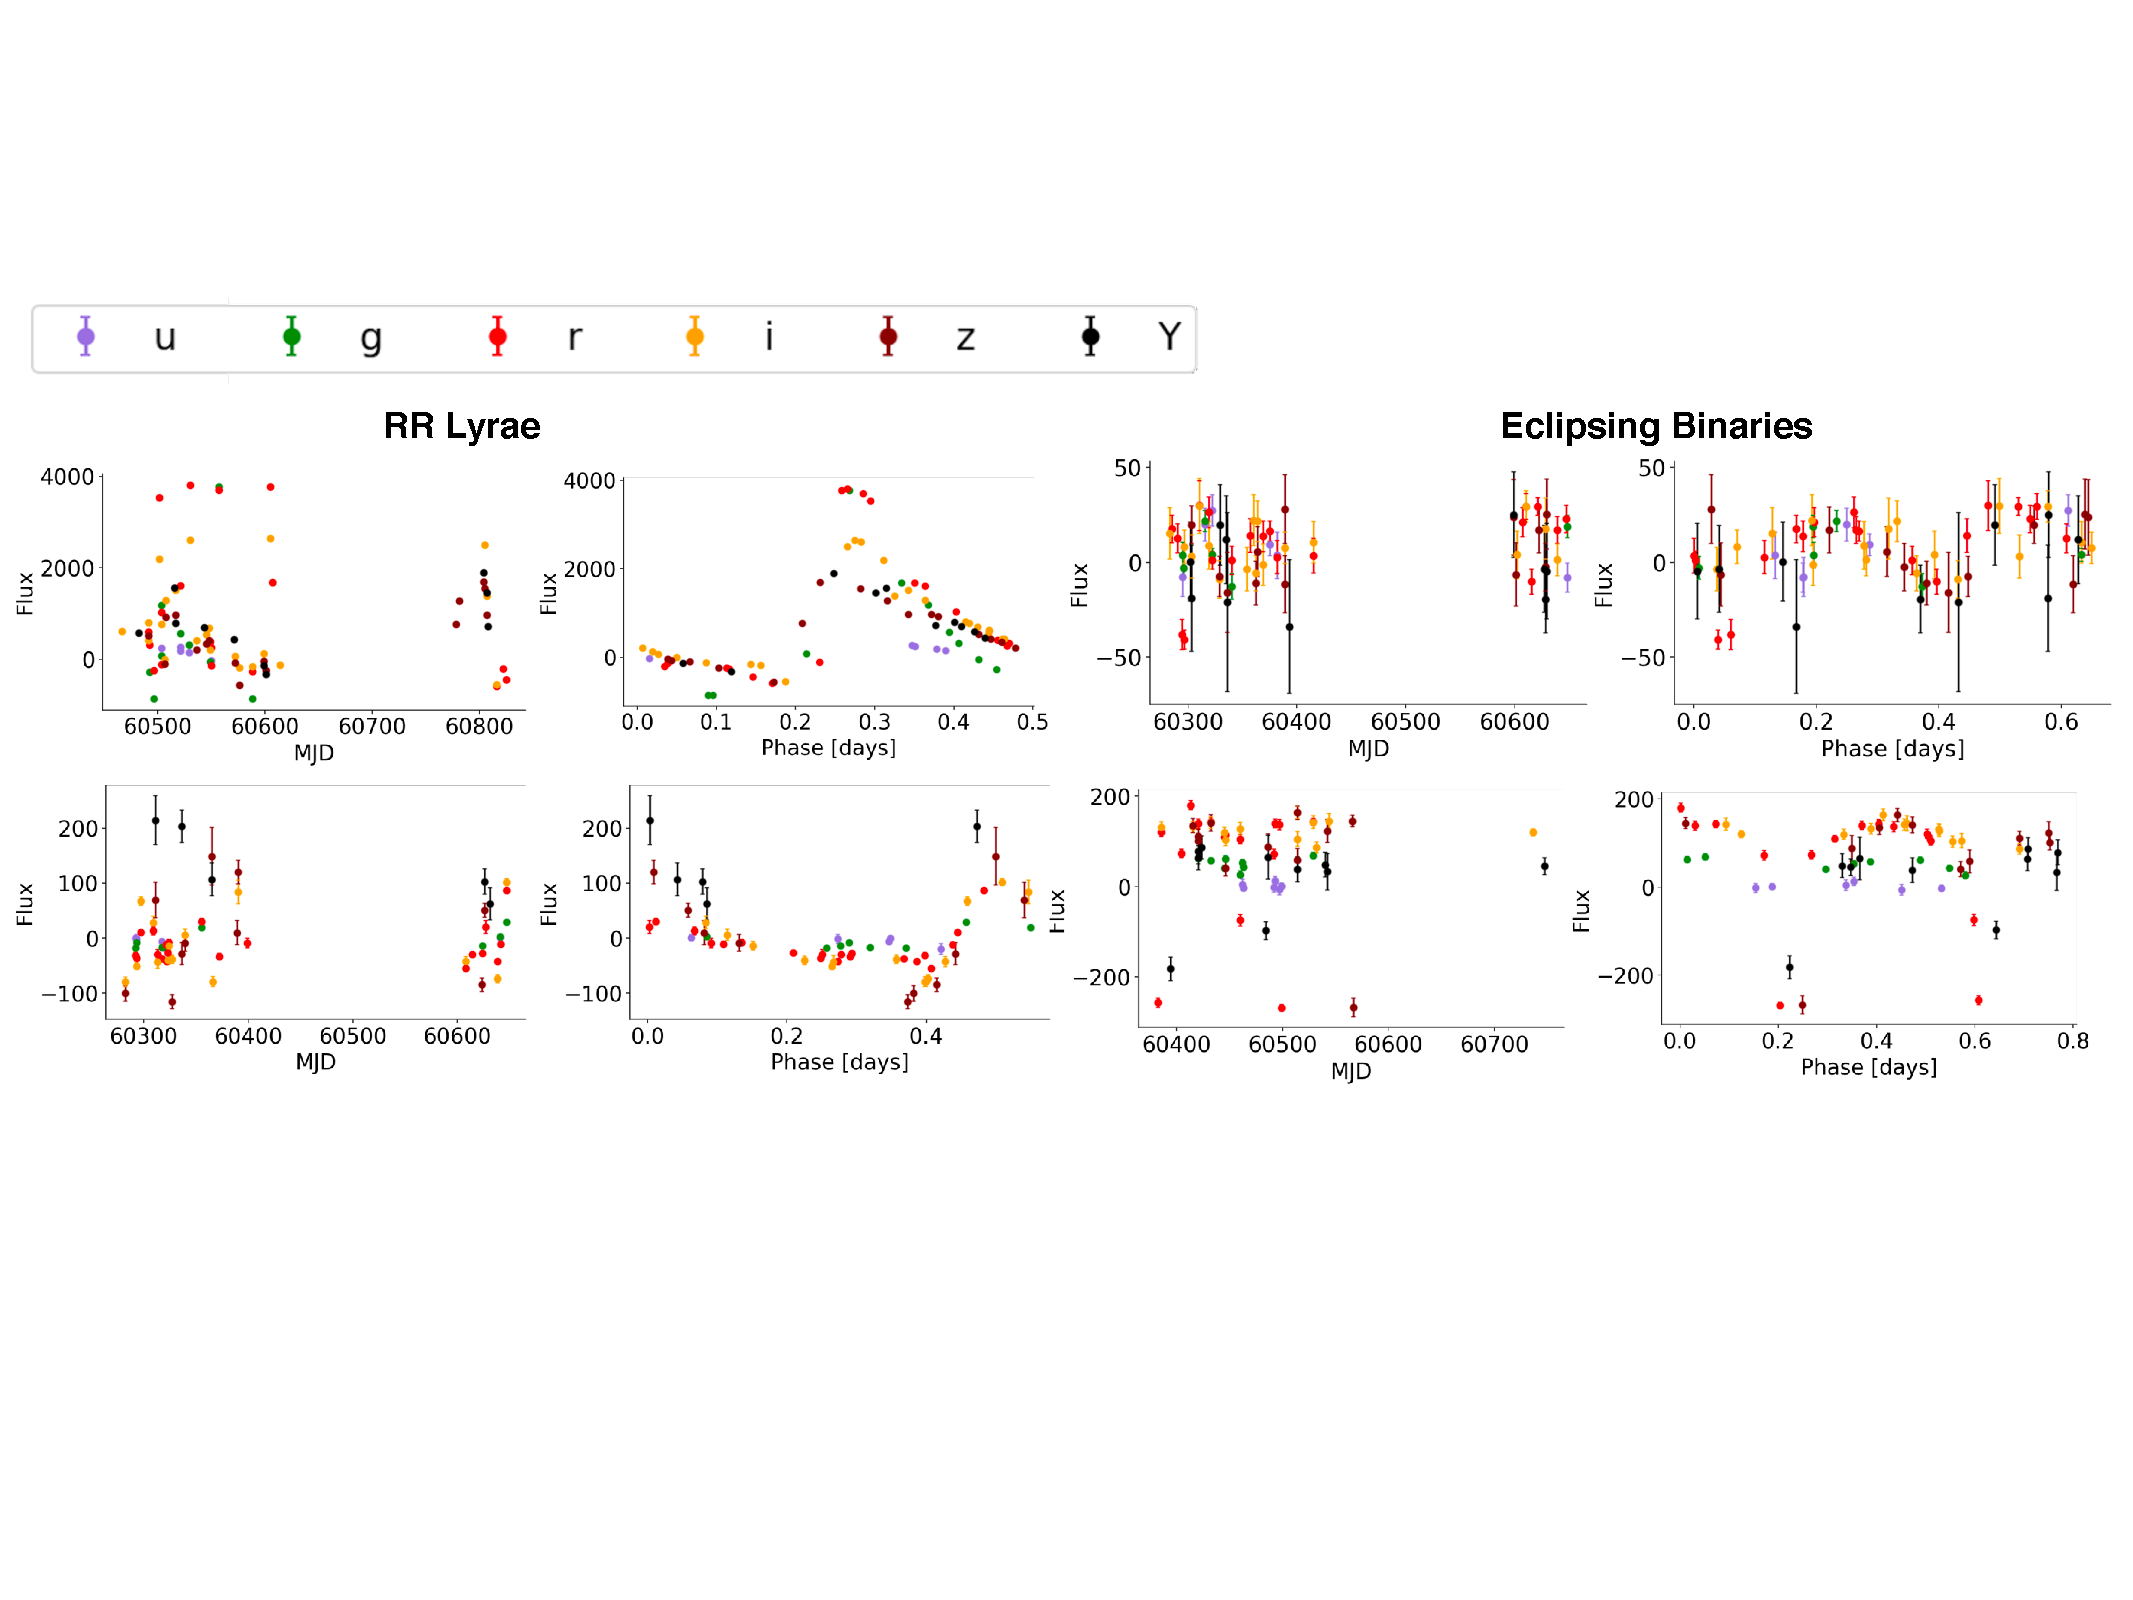
\includegraphics[width=0.9\textwidth]{figures/lightcurve_demo.pdf}
  \centering 
  \caption{The above panels demonstrate the multi-band light curves simulated from ElasTiCC using RR lyrae (left panel) and eclipsing binaries (right panel). The first column of each panel shows the observed light curves, and the second the phase folded light curves at the correct period after 12 months.}
   \label{fig:light_curve_demo}
\end{figure*}


\section{Injection-Recovery Testing}
We consider two models of periodic phenomena: RR lyrae and eclipsing binaries ranging from a periods of 0.2 days to 10 days. All computations of the floating-mean Lomb-Scargle periodogram are using the open-source Python package `gatspy` \citet{VanderPlas:VP2015}. 


\subsection{Single Band Lomb-Scargle Periodogram}

We first consider the case of single-band detections from AP. Here we aim to answer if the 12 month AP history in a single-band light curve is enough to recover periods. We consider the canonical floating mean to estimate the periodogram of 10,000 alert light curves in the $r$-band for three Fourier component modes. In Figure \ref{fig:single_band_lsp} we show the results of this analysis for RRL's (rop row) and EB's (bottom row). For each light curve model, we randomly sample a light curve and compute the Lomb-Scargle periodogram using a heuristic period grid with an oversampling factor of 2 and Nyquist frequency of 30 ($\sim$0.03 days) to account for the fast periodic phenomena. We extrapolated the highest power period from the periodogram and compare it to the true period. In Figure \ref{fig:single_band_lsp} we also include the number of $r$-band detections for each light curve. As expected, we did not find any preference of an optical single-band photometric filter that outperformed the others. While the RR Lyrae exhibit at larger Fourier modeling modes more aliasing, overall the recovery fraction of correctly identified periods is larger compared to the EBs. For both light curve models, we consistently found in each model configuration that the average correctly identified period coincides with a larger number of detections. Overall we find consistent results for the RR Lyrae done by a similar analysis by \citet{VanderPlas:VP2015}. The true challenge of this approach comes from the more complex light curves such as the EBs. 


On average, there will be 30 detections in each band per 12 month light curve history. This entails that the majority of AP light curves will likely be too undersampled in order to compute a high confidence periodicity. 


% Todo
\begin{itemize}
\item Injected vs recovered period plots eclipsing binaries and RRL
\item Fraction of correctly recovered periods using single-band Lomb-Scargle (for N=1...3 Fourier components)  
\end{itemize}

\begin{figure*}
  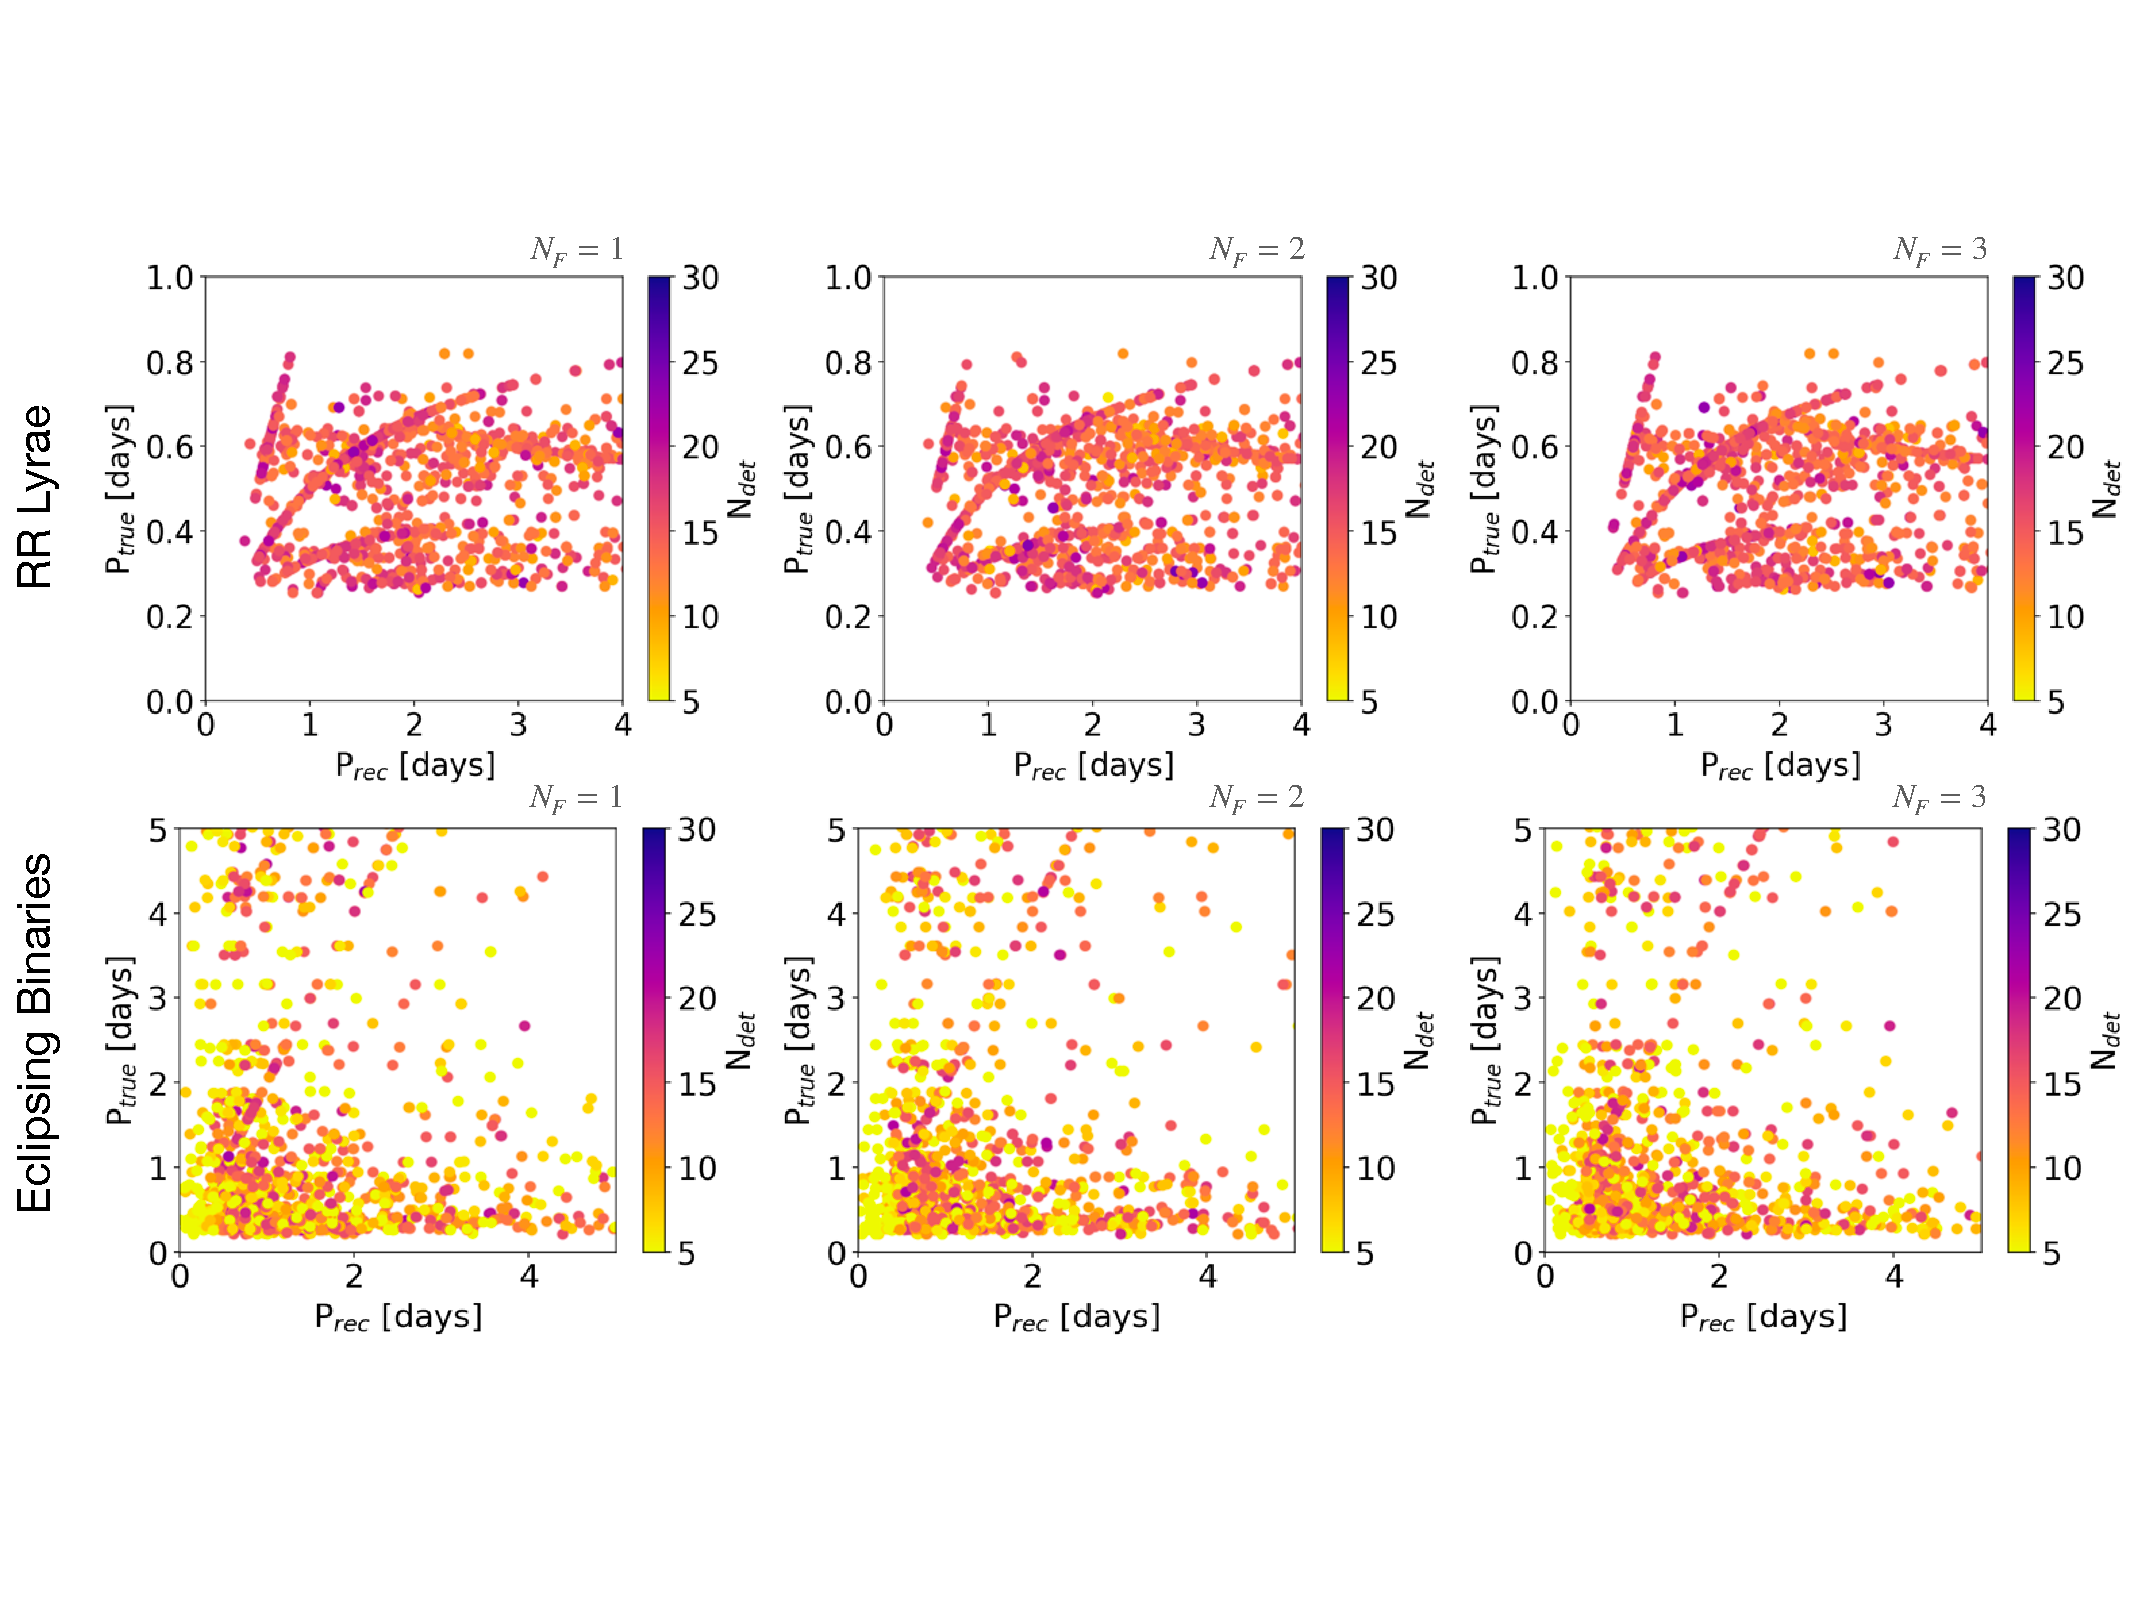
\includegraphics[width=0.8\textwidth]{figures/singleband_lsp.pdf}
  \centering 
  \caption{We show the injected (true period) versus recovered highest peak in the periodogram for a sample of 1000 $r$-band detections from RR lyrae and eclipsing binaries. Each column shows the period recovery for N=1 to N=3 Fourier components when computing the Lomb-Scargle periodogram.}
  \label{fig:single_band_lsp}
\end{figure*}

% Conclusions regarding the single-band Lomb Scargle
Even with a low completeness, computing the Lomb-Scargle periodogram on single-band time series alerts, this will likely outperform any other known survey due to the large survey volume. Single-band Lomb-Scargle implementations are also faster by a factor of $\sim$5 due to the lower average number of detections per filter. Given that only roughly 17 percent of each bandpass filter will be available, the single-band Lomb-Scargle misses by a higher margin the underlying true period. We now turn our attention to the multi-band Lomb-Scargle.

\subsection{Multi-Band Lomb-Scargle Periodogram}

Next, we test the multi-band Lomb-Scargle periodogram implementation adapted on \textit{gatspy} to our ELAsTiCC light curves. Given the rich multi-band alert detections LSST will deliver, we expect that that conventional period finding algorithms will perform better. Generally, the multi-band Lomb-Scargle periodogram we will be considering for this study can be written out with two components: 

\begin{equation}
\qquad y = theta_0+\sum_{n=1}^{M_{base}}\left[\theta_{2 n-1} \sin (n \omega t)+\theta_{2 n} \cos (n \omega t)\right] \\
\theta_0^{(k)}+\sum_{n=1}^{M _{band}}\left[\theta_{2 n-1}^{(k)} \sin (n \omega t)+\theta_{2 n}^{(k)} \cos (n \omega t)\right]
\end{equation}

First is the base Fourier component that describes the overall \textbf{shared} variability, and second is the per band component that is modeled by the residuals of the base component with each photometric filter. In practice, a larger configuration of base and band components can lead to the estimation of more complex light curves. \textit{Gatspy} automatically determines through the use of least-squares minimization the scalar parameters from the above equation. 

\begin{figure*}
  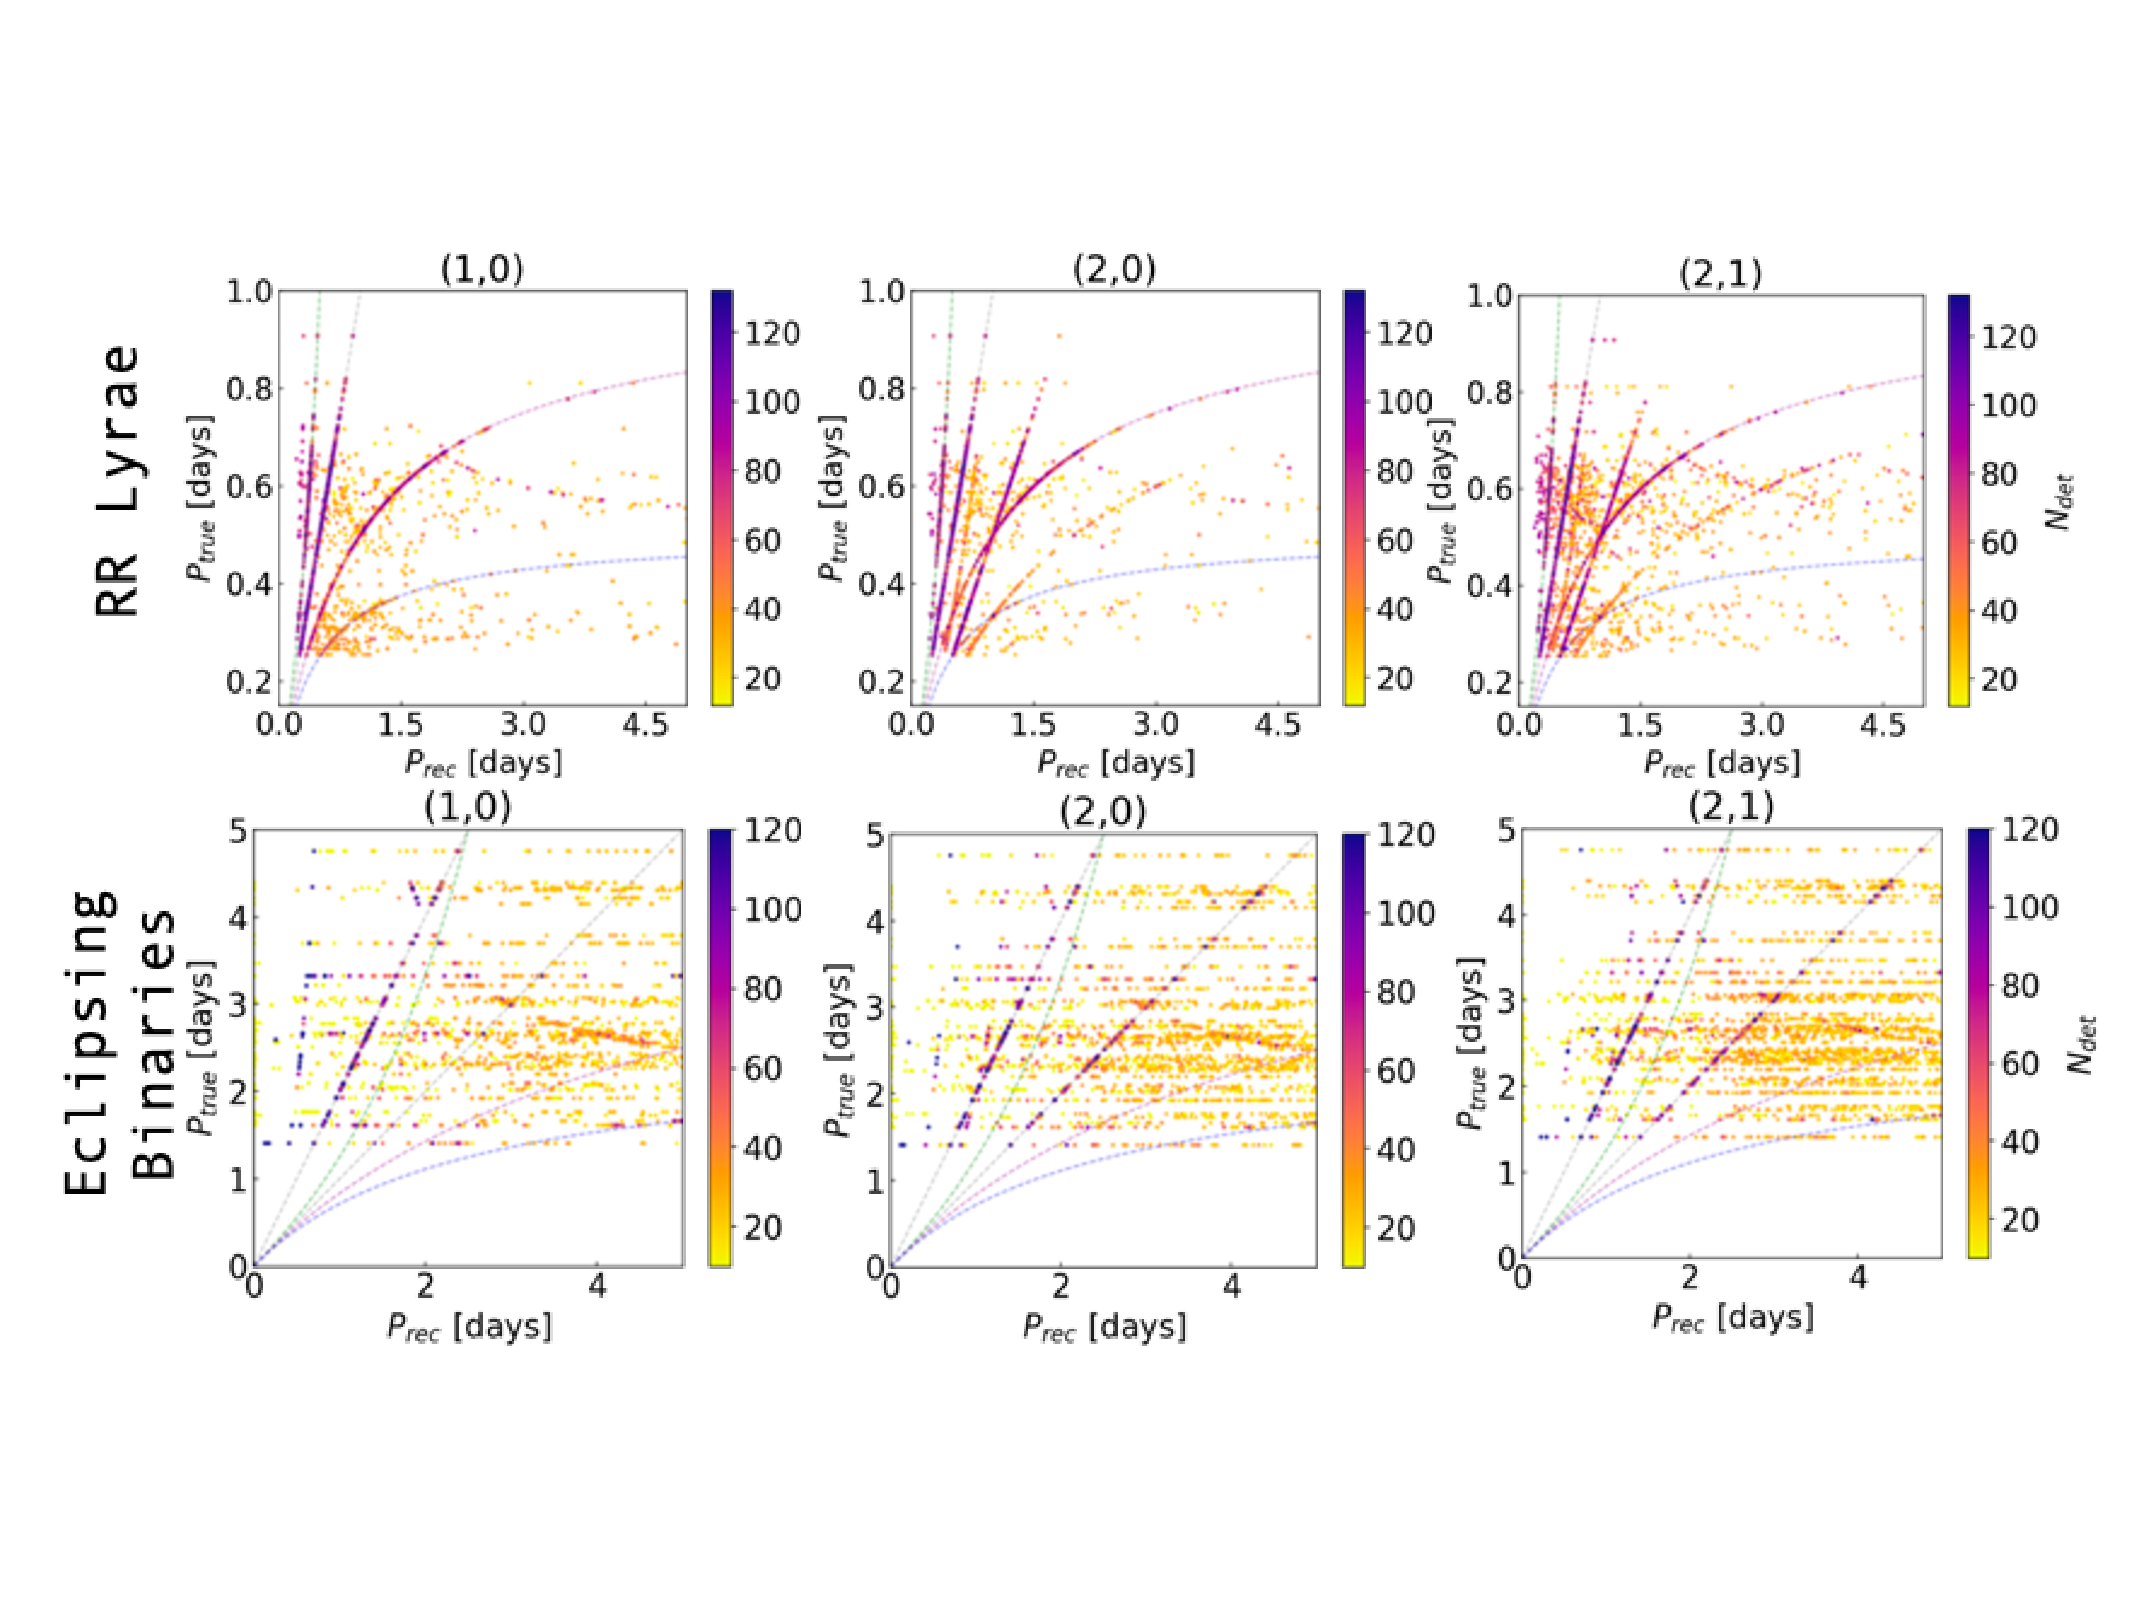
\includegraphics[width=0.9\textwidth]{figures/multi_lsp_rectest.pdf}
  \centering 
  \caption{Multi-band injection-recovery test for 5000 RRL (top row) and EB (bottom row). Each column title includes the number of Fourier base and band terms used to compute the Lomb-Scargle periodogram. Additionally we color code each recovered period by the number of detections. The overlaid curved lines represent the n=1 aliasing, while the straight lines represent the n=1,2 harmonics.}
\end{figure*}

Figure for comparing each method

\begin{figure*}
  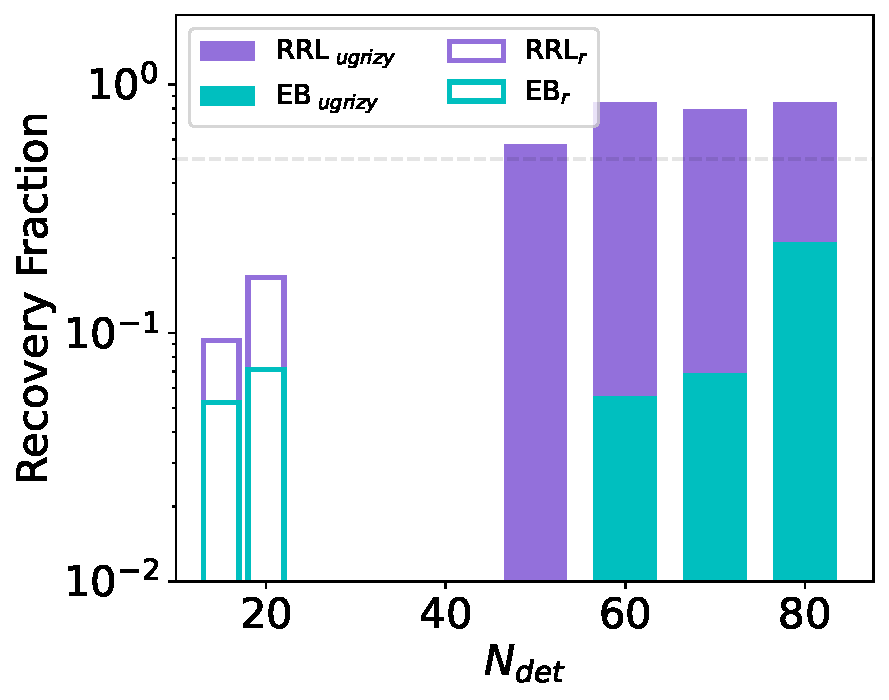
\includegraphics[width=0.6\textwidth]{figures/multi_vs_single_rec_frac.pdf}
  \centering 
  \caption{Multi-band injection-recovery test for 5000 RRL (top row) and EB (bottom row). Each column title includes the number of Fourier base and band terms used to compute the Lomb-Scargle periodogram. Additionally we color code each recovered period by the number of detections. The overlaid curved lines represent the n=1 aliasing, while the straight lines represent the n=1,2 harmonics.}
\end{figure*}



\subsection{Period Grid}
The LSST will be search for periodic phenomena across both short and long timescales. Another challenge is choosing the right trial period grid with separations that can lead to successful period finding within AP. The periodogram is full of local minima and maxima, thus in practice the global maximum, which corresponds usually to the period with the highest power, is searched through 

Inevitably, large searches in period space without an a priori will require an heuristic approach to generating an appropriate period grid that will account for the light curve characteristics. 

For this study, we use a heuristic frequency grid generator adapted in gatspy that uses the light curve parameters to estimate the appropriate frequency grid length and separation. Generally, the frequency separation can be approximated using the duration of the light curve, including some sampling constant ($\mathcal{O}$):
\begin{equation}
\delta f = \frac{1}{(t_{max} - t_{min}) \times \mathcal{O}}
\end{equation}

and the total number of computed periods as a function of the Nyquist frequency ($F_{nyquist}$), and number of detections (N$_{det}$): 
\begin{equation}
N_{P} = int \bigg{(} \frac{1}{2} \mathcal{O} F_{nyquist} N_{det} \bigg{)}
\end{equation}

Intuitively, the Nyquist frequency pushes the minimum starting frequency to smaller periods, while the oversampling factor will increase the maximum frequency grid and overall increase the coarseness of the grid. In later sections we evaluate for each frequency grid the period accuracy computed for the ELAsTiCC light curves. 

\subsection{Peak Significance Metric}

In this section we discuss possible metrics for peak significance. One challenge when computing the periodogram for billions of sources is the inevitability of spurious period detections, effects of harmonics, and aliasing. One diagnostic used in the literature is the False Alarm Probability (FAP) of a given peak in the power spectrum. The FAP measures the probability uncertainty associated with the selected peak under the null hypothesis.

% What is the FAP we want to measure here? Bootstraping is a proxy to FAP... 

\begin{figure*}
  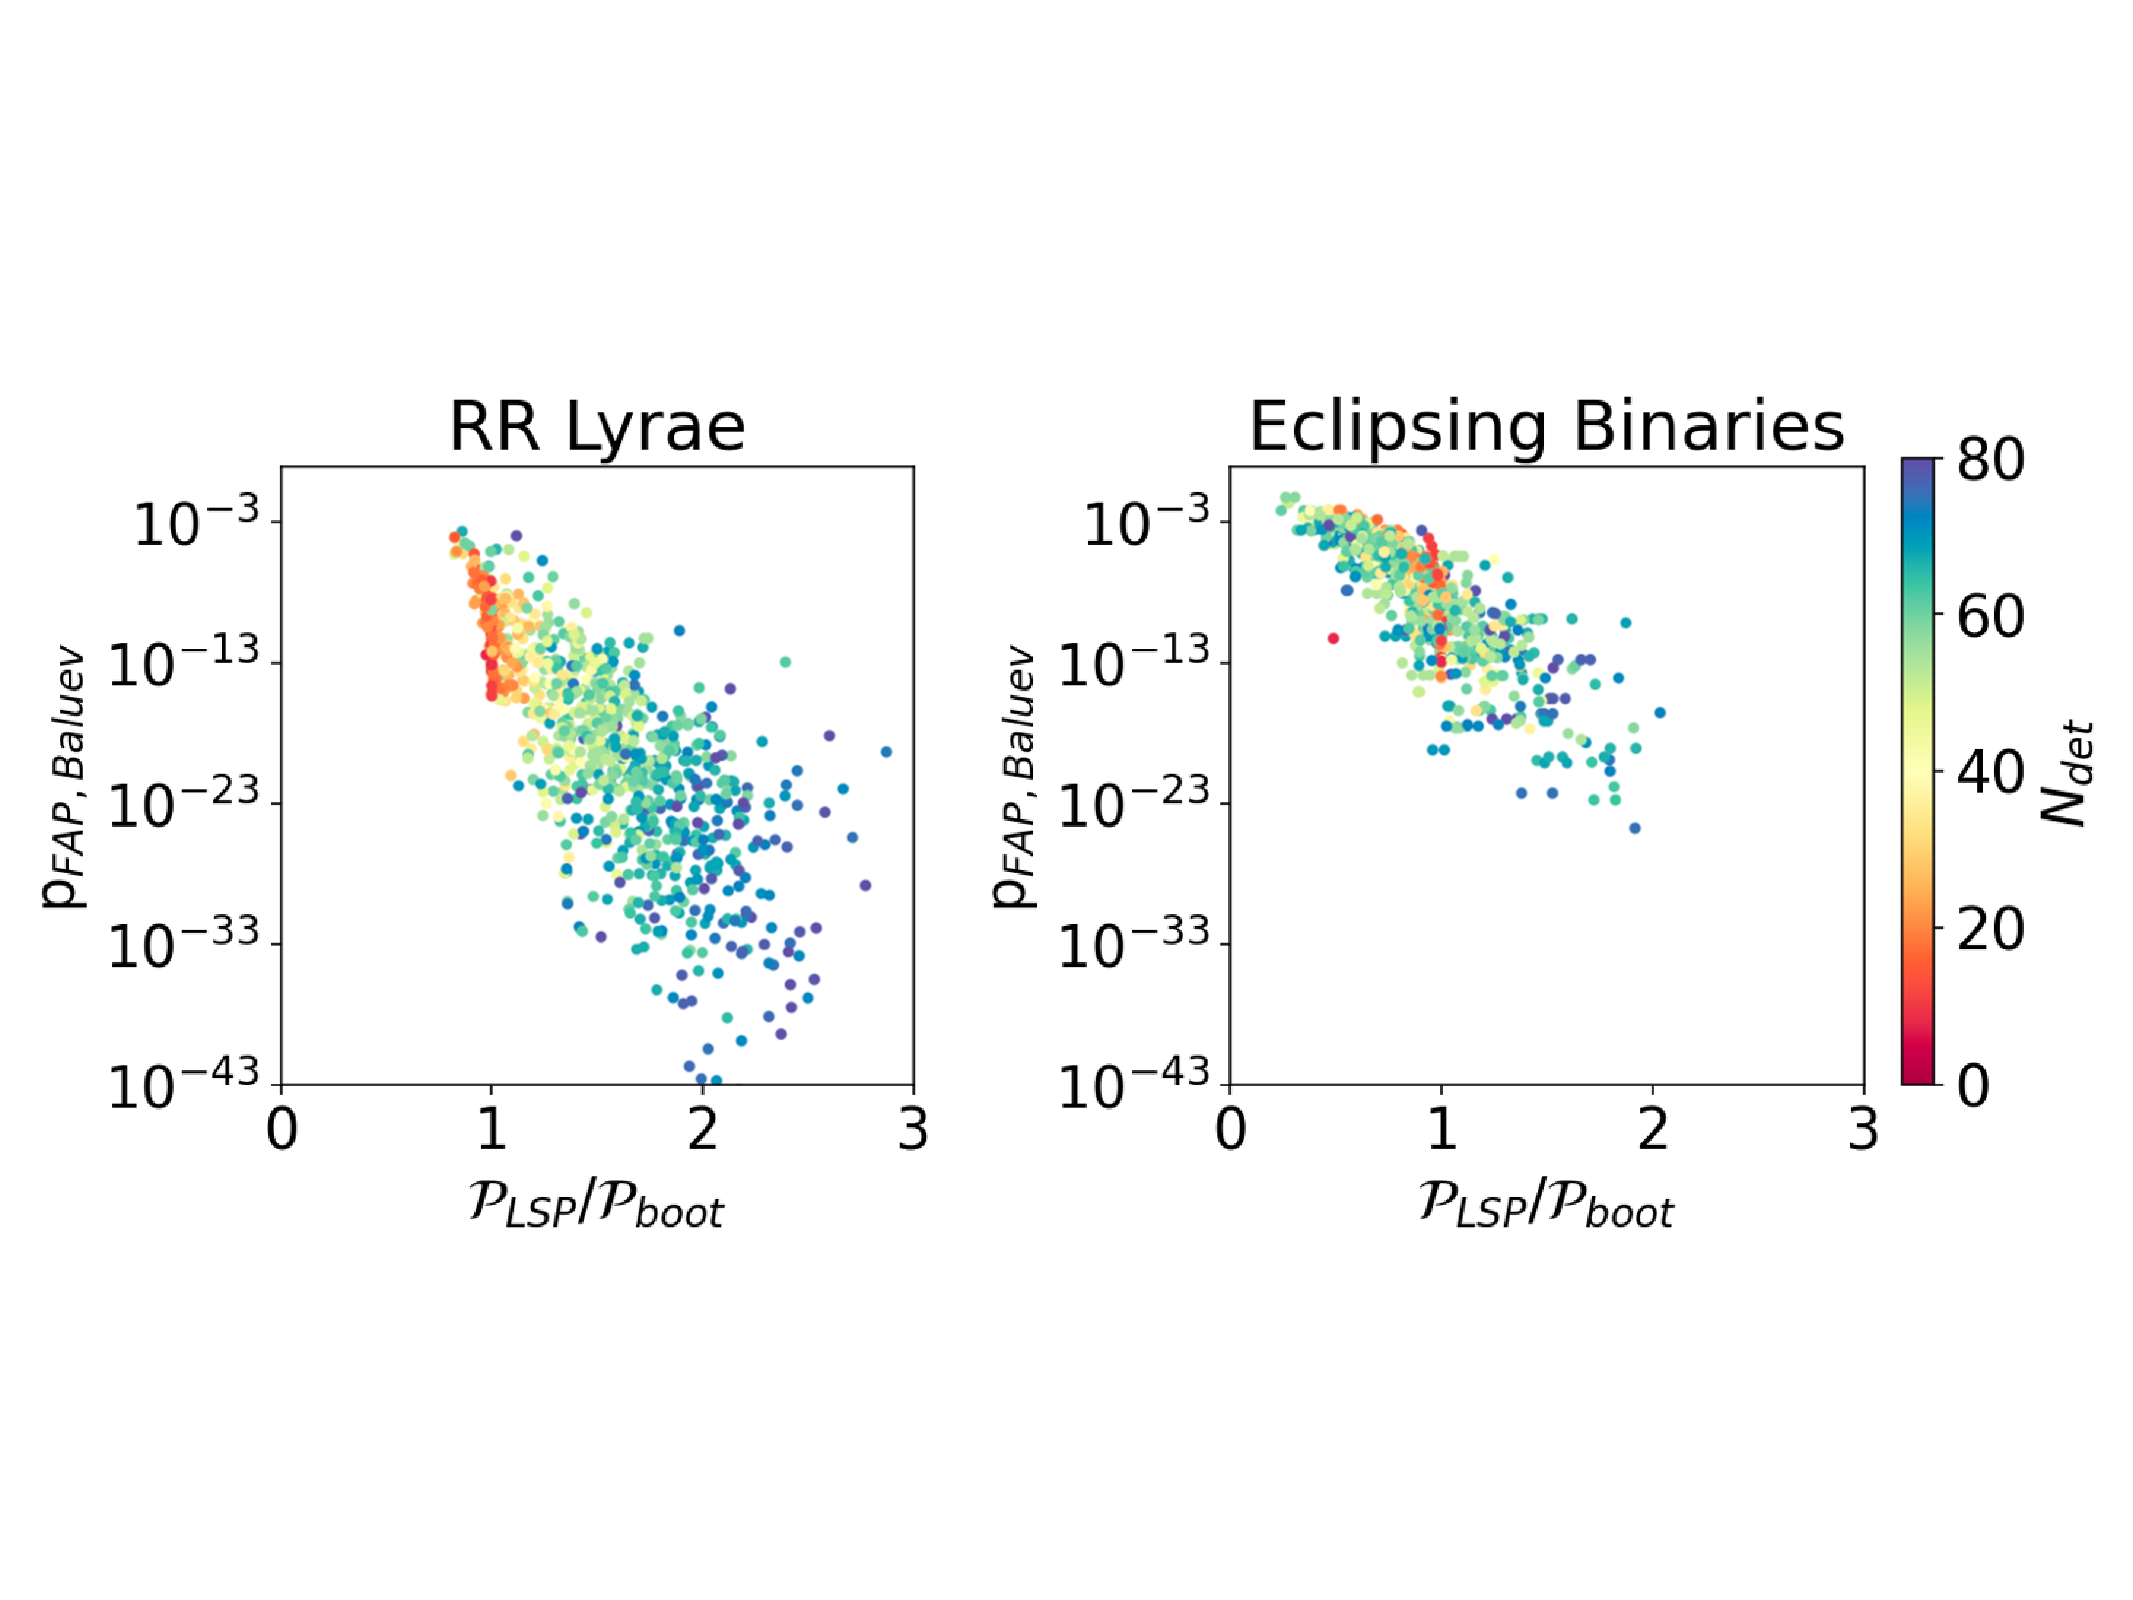
\includegraphics[width=0.8\textwidth]{figures/fap_approximation_mlsp.pdf}
  \centering 
  \caption{Multi-band FAP rate computed via the Baluev approximation compared to a $2\sigma$ bootstrap approach for 5000 RRL and EB alert light curves. For each light curve we also color code the total number of $ugrizy$ detections.}
\end{figure*}

We will be using the approximation of the Baluev form:
\begin{equation}
P_{FAP} \approx \frac{\Gamma((N-1) / 2)}{\Gamma((N-2) / 2)} \sqrt{4 \pi \operatorname{var}\left(t_i\right)} f_{\mathrm{u}}\left(1-z_{\mathrm{obs}}\right)^{\frac{N-4}{2}} \sqrt{z_{\mathrm{obs}}}
\end{equation}


% Summary: Timing analysis will include details on bench marking the run time of each frequency grid and model as a function of number of detections and period accuracy.
\subsection{Timing Analysis}

% Introduction
In this section we bench mark the average run time of the Lomb-Scargle periodogram implementation from gatspy. The balancing act of high periodocity accuracy while confining the calculations within the AP timeframe is a challenging act. While coarse period grids  and complex models can achieve more accurate periods, this will not be possible to do with AP. Instead, in this section we will explore the lower limit of run time while tweaking the overall period grid coarseness and model complexity.

The current gatspy, which is a pure Python based implementation of the Lomb-Scargle periodogram, scales as  $\mathcal{O}$[N] algorithm for small N and becomes $\mathcal{O}$[N$^2$] at larger trial periods. The unique rapid calculation of the periodogram emerges from the efficient use of linear algebraic operations. The average run time also depends on the number of detections and model complexity which we will explore in this section. For our run time analysis we will consider both a single-band and multi-band case for the RR Lyrae only since the run time is not a function of the underlying signal. 

% Discussion of single-band 
We first measure the effects of run time on the single-band RRL photometry in the $r$-band filter. In practice, this would work for any given filter given the rolling cadence of LSST. For each light curve, we run the Lomb-Scargle periodogram 10 times per light curve, and compute the median run time. Additionally, we run this for each combination of oversampling factor, Nyquist frequency, and Fourier components. In Figure \ref{fig:run_time_single}, we display the results for the single-band photometry. We also color code the average fractional error per light curve iteration. As mentioned in the single-band Lomb-Scargle method, by design will be poorly sampled especially within the 12 month history. As expected, due to the sparse sampled light curves, the majority of light curves scale linearly with number of detections, and have average run times below one second. 


 
 \begin{figure*}
  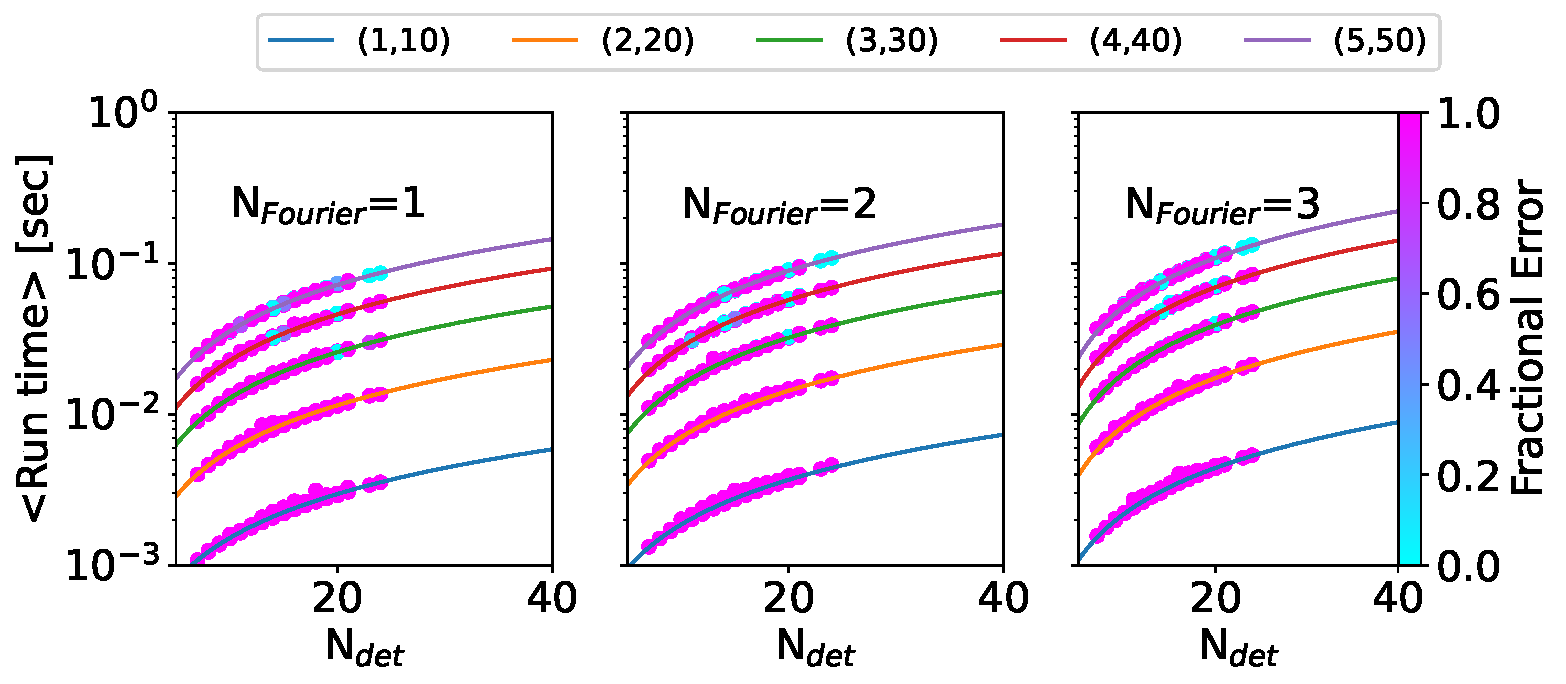
\includegraphics[width=0.8\textwidth]{figures/singleRUN_LSP_RRL.pdf}
  \centering 
  \caption{Average run time per number of $r$ light curve detections. Each column represents the model complexity of each multi-band Lomb Scargle periodogram. Within each panel, we use a heuristically determined period grid by varying the oversampling factor and the the Nyquist frequency.  Finally, for each successive run we color code the fractional error compared from the true period.}
  \label{fig:run_time_single}
\end{figure*}

% Discussion of multi-band

% Conclusions & recommendations  



\begin{figure*}
  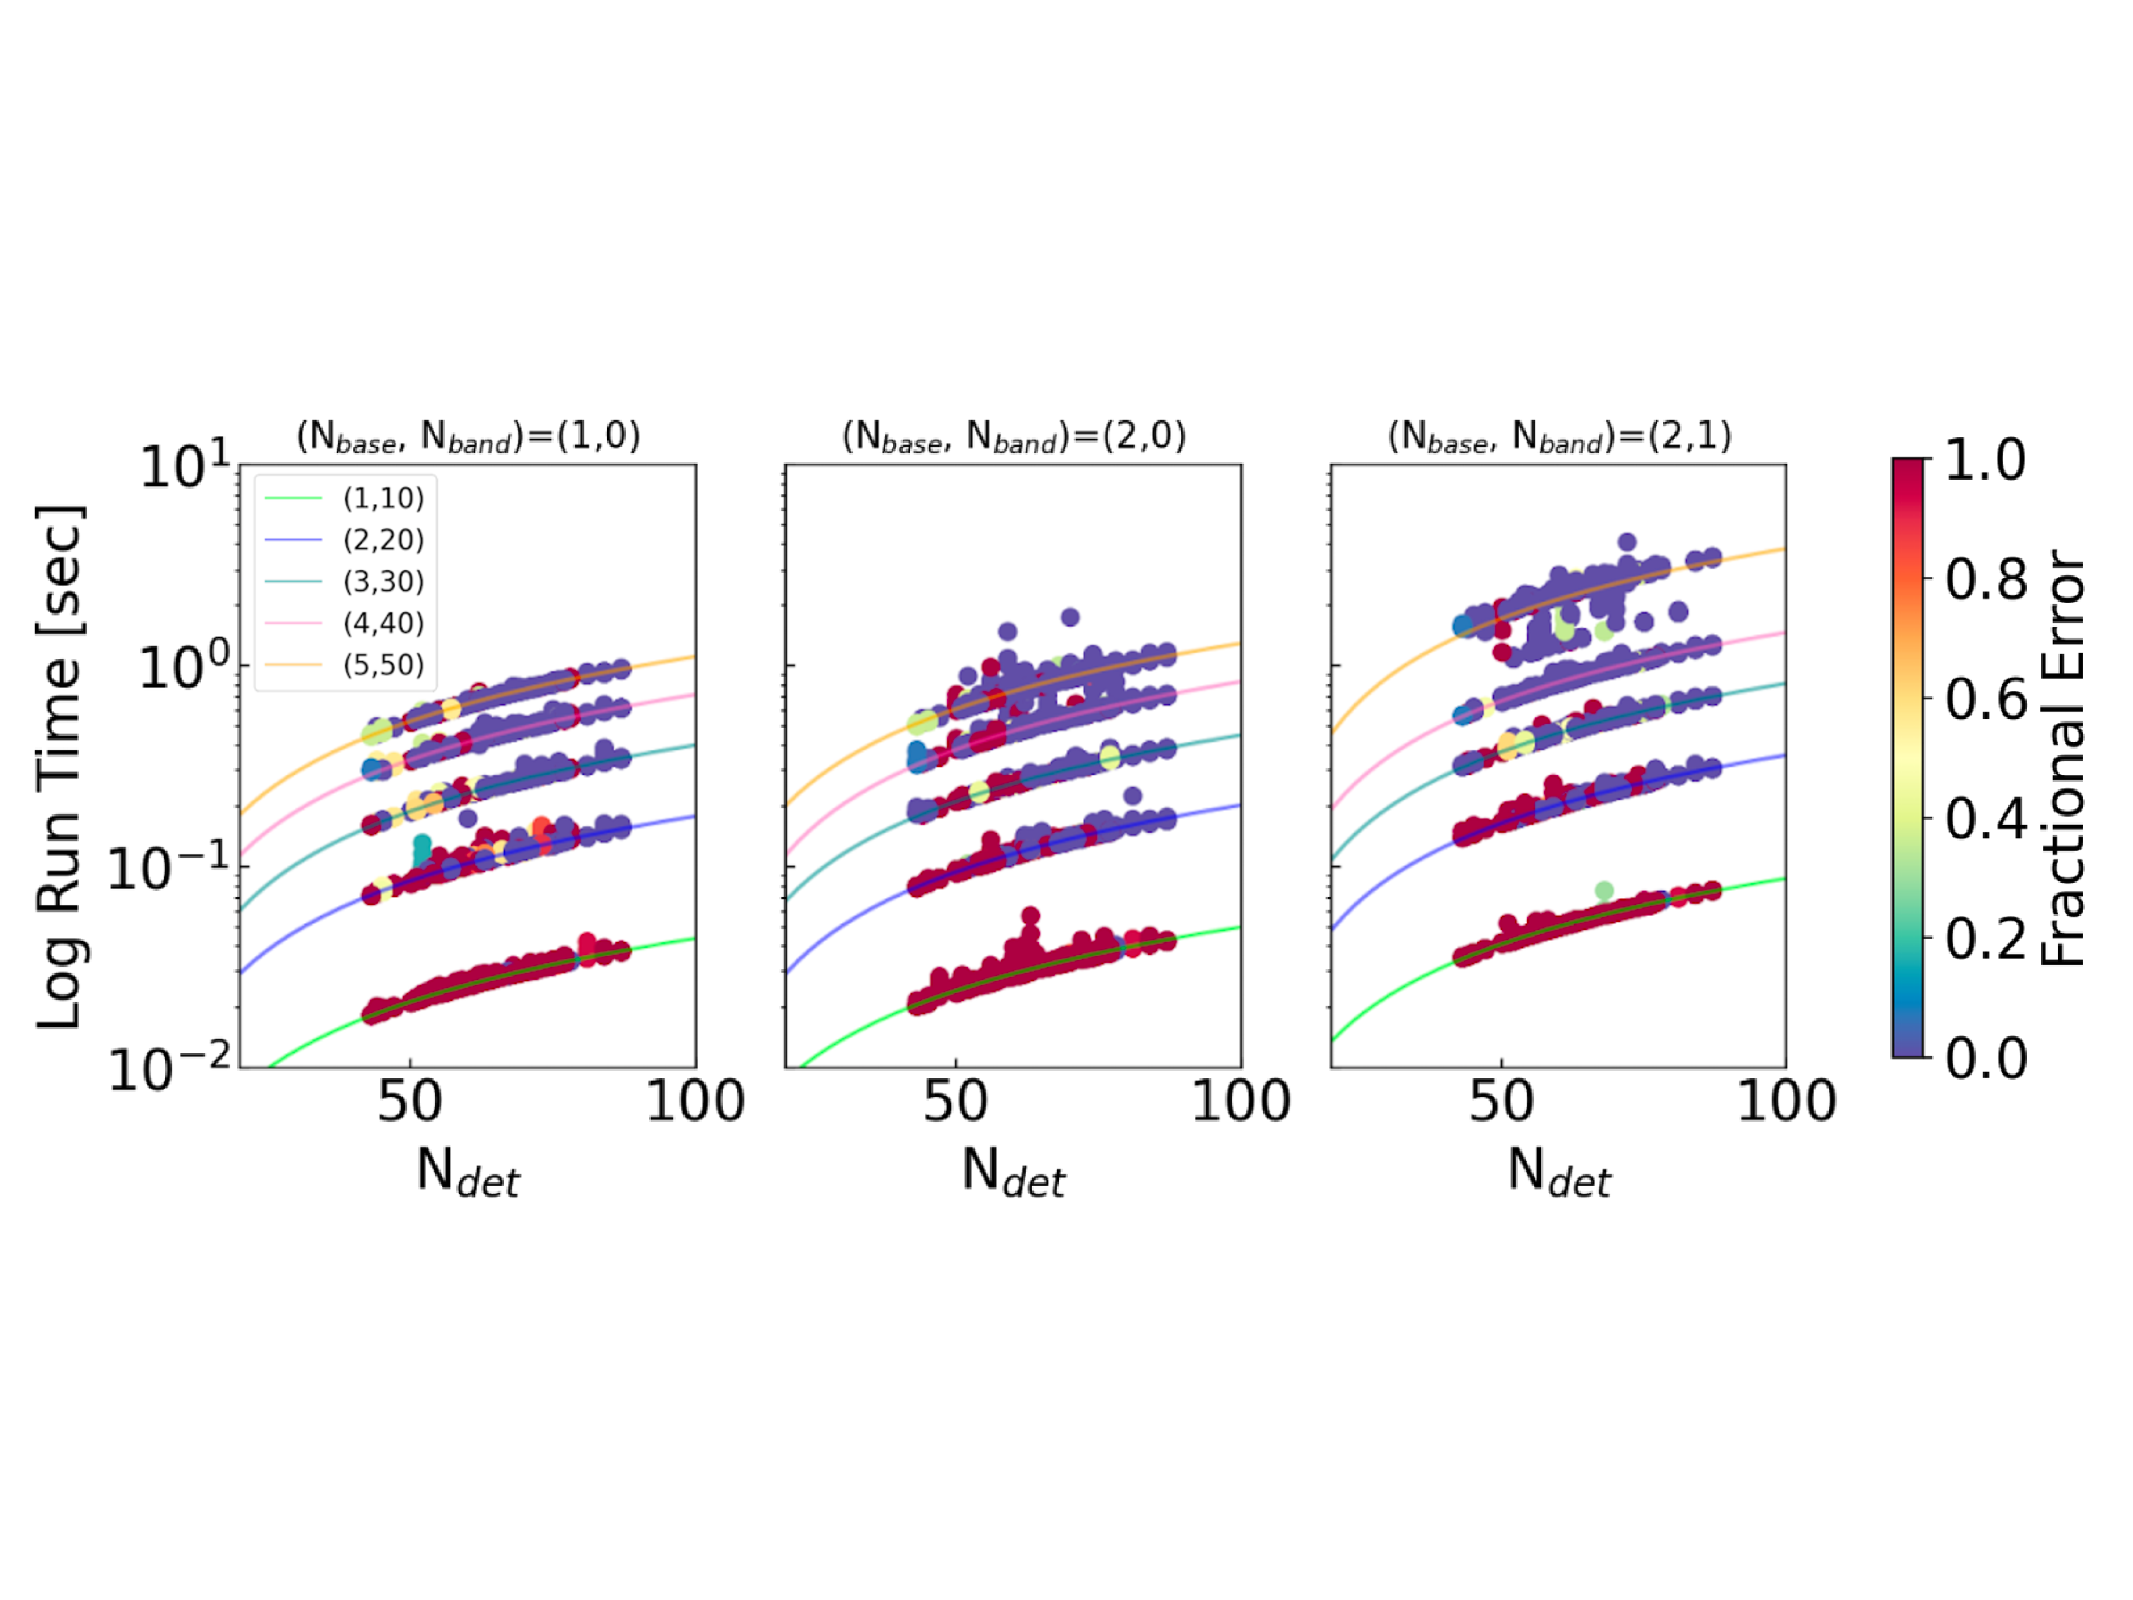
\includegraphics[width=0.8\textwidth]{figures/run_time_analysis.pdf}
  \centering 
  \caption{Average run time per number of $ugrizy$ light curve detections. Each column represents the model complexity of each multi-band Lomb Scargle periodogram. Within each panel, we use a heuristically determined period grid by varying the oversampling factor and the the Nyquist frequency.  Finally, for each successive run we color code the fractional error compared from the true period.}
\end{figure*}


\appendix
% Include all the relevant bib files.
% https://lsst-texmf.lsst.io/lsstdoc.html#bibliographies
\section{References} \label{sec:bib}
\bibliography{local,lsst,lsst-dm,refs_ads,refs,books}

% Make sure lsst-texmf/bin/generateAcronyms.py is in your path
\section{Acronyms} \label{sec:acronyms}
\addtocounter{table}{-1}
\begin{longtable}{p{0.145\textwidth}p{0.8\textwidth}}\hline
\textbf{Acronym} & \textbf{Description}  \\\hline

AGN & active galactic nuclei \\\hline
CCD & Charge-Coupled Device \\\hline
DC2 & Data Challenge 2 (DESC) \\\hline
DIA & Difference Image Analysis \\\hline
DM & Data Management \\\hline
DMTN & DM Technical Note \\\hline
EB & ExaByte \\\hline
HR & Human Resources \\\hline
LSST & Legacy Survey of Space and Time (formerly Large Synoptic Survey Telescope) \\\hline
SDSS & Sloan Digital Sky Survey \\\hline
\end{longtable}






\end{document}
